\documentclass[10pt]{article}

\addtolength{\oddsidemargin}{-.875in}
\addtolength{\evensidemargin}{-.875in}
\addtolength{\textwidth}{1.75in}

\addtolength{\topmargin}{-.875in}
\addtolength{\textheight}{1.75in}

\openup 1em

%macro for commenting
\usepackage{color}
\newcommand{\leo}[1]{{\color{blue}{LD: #1}}}

% \newcommand{\Xbeta}{ X_i \theta}
\newcommand{\xbeta}{ x_i \beta}
\newcommand{\xtheta}{ x_i \theta}
% \newcommand{\xbetaij}{ x_{ij}^T \theta}
\newcommand{\sgamma}{s_{ij}^T\gamma_i}

\usepackage[round]{natbib}

\usepackage{rotating}
\usepackage{graphicx}
\usepackage{subcaption}

\usepackage{float}
\usepackage{bbm}

\usepackage{amsthm,amsmath, amssymb} 
\usepackage{mathrsfs}
\usepackage{subcaption}
\usepackage{nicefrac}

\newtheorem{theorem}{Theorem}
\newtheorem{lemma}{Lemma}
\newtheorem{corollary}{Corollary}
\newtheorem{remark}{Remark}


\usepackage{algorithm}
\usepackage{algpseudocode}

%\usepackage{mhequ}
\newcommand{\be}{\begin{equation}\begin{aligned}}
\newcommand{\ee}{\end{aligned}\end{equation}}
\newcommand{\bb}[1]{\mathbb{#1}}
\newcommand{\mc}[1]{\mathcal{#1}}
\DeclareMathOperator{\Binom}{Binomial}
\DeclareMathOperator{\No}{No}
\DeclareMathOperator{\PG}{PG}
\DeclareMathOperator{\IG}{Inverse-Gamma}
\DeclareMathOperator{\Ga}{Gamma}
\DeclareMathOperator{\Bern}{Bernoulli}
\DeclareMathOperator{\U}{Uniform}
\DeclareMathOperator{\Poi}{Poisson}
\DeclareMathOperator{\NB}{NB}
\DeclareMathOperator{\cov}{cov}
\DeclareMathOperator{\var}{var}
\DeclareMathOperator{\diag}{diag}
\DeclareMathOperator{\Diag}{Diag}
\newcommand{\KL}[2]{\textnormal{KL}\left(#1 \parallel #2\right)}

\DeclareMathOperator{\1}{\mathbbm{1}}


\DeclareMathOperator{\bigO}{\mc O}



\thispagestyle{empty}
\baselineskip=28pt

\title{\textbf{Extrinsic Priors for Bayesian Modeling with Parameter Constraints}}
\author{Leo Duan, Akihiko Nishimura, David Dunson}
\date{}
\begin{document}
\maketitle
{\bf Abstract:} Prior information often takes for the form of parameter constraints. Bayesian methods include such information through prior distributions having constrained support. By using posterior sampling algorithms, one can quantify uncertainty without relying on asymptotic approximations. However, outside of narrow settings, parameter contraints make it difficult to develop efficient posterior sampling algorithms. We propose a general solution, which relaxes the constraint through the use of an {\em extrinsic prior}, which is concentrated close to the constrained space. General off the shelf posterior sampling algorithms, such as Hamiltonian Monte Carlo (HMC), can then be used directly. We illustrate this approach through multiple examples involving equality and inequality constraints. While existing methods tend to rely on conjugate families, our proposed approach frees us up to define new classes of hierarchical models for constrained problems. We illustrate this through application to a variety of simulated and real datasets.
\vskip 12pt
%\baselineskip=12pt
%\par\vfill\noindent
{\noindent KEY WORDS: Constraint relaxation; Euclidean Embedding; Monotone Dirichlet; Soft Constraint; Stiefel Manifold; Projected Markov chain}
%\par\medskip\noindent
%\clearpage\pagebreak\newpage
\pagenumbering{arabic}


\section{Introduction}
It is extremely common to have prior information available on parameter contraints in statistical models. For example, one may have prior knowledge that a vector of parameters lies on the probability simplex or satisfies a particular set of inequality constraints. Other common examples include shape constraints on functions, positive semidefiniteness of matrices and orthogonality. There is a very rich literature on optimization subject to parameter contraints. One common approach is to rely on Langrange and Karush-Kuhn-Tucker multipliers \citep{boyd2004convex}. However, simply producing a point estimate is often insufficient, as uncertainty quantification (UQ) is a key component of most statistical analyses. Usual large sample asymptotic theory, for example showing asymptotic normality of statistical estimators, tends to break down in constrained inference problems. Instead, limiting distributions may have a complex form that needs to be rederived for each new type of constraint, and may be intractable. An appealing alternative is to rely on Bayesian methods for UQ, including the constraint through a prior distribution having restricted support, and then applying Markov chain Monte Carlo (MCMC) to avoid the need for large sample approximations.

Conceptually MCMC can be applied in a broad class of constrained parameter problems without complications \cite{gelfand1992bayesian}. However, in practice, a primary difficulty is designing a Markov transition kernel that leads to an MCMC algorithm with sufficient computational efficiency to be practically useful. Common default transition kernels correspond to Gibbs sampling, random walk Metropolis-Hastings, and (more recently) Hamiltonian Monte Carlo (HMC). Gibbs sampling relies on alternately sampling from the full conditional posterior distributions for the different parameters, ideally in blocks to improve mixing. Gibbs requires the conditional distributions to be available in a form that is tractable to sample from directly, limiting consideration to specialized models. In constrained problems, block updating is typically either not possible or very inefficient (e.g. relying on rejection sampling with a high rejection probability), and one-at-a-time updating can lead to extremely slow mixing. Random walk algorithms provide an alternative, but each step of the random walk must maintain the parameter constraint. A common approach is to apply a normal random walk and simply reject proposals that violate the constraint, but this can have very high rejection rates even if using an adaptive approach that learns the covariance based on the history of the chain. An alternative is to rely on HMC. In simple settings in which a reparameterization can be applied to remove the constraint, HMC can be applied easily. Otherwise, HMC will generate proposals that violate the constraint, and hence face problems with high rejection rates in heavily constrained problems.

Due to the above hurdles, most of the focus in the literature has been on customized solutions developed for specific constraints.
One popular strategy is to carefully pick a prior and likelihood such that posterior sampling is tractable. For example, for modeling of data on manifolds, it is typical to restrict attention to specific models, such as the Bingham-von Mises-Fisher distribution for Stiefel manifolds \citep{khatri1977mises,hoff2009simulation}. For data on the probability simplex, one instead relies on the Dirichlet distribution. An alternative is to reparameterize the model to eliminate or simplify the constraint. For example, when faced with a monotonicity constraint, one may reparameterize in terms of differences as the resulting positivity constraint leads to much easier sampling (REFs). In the literature on modeling of data on manifolds, there are two strategies: (i) {\em intrinsic} methods that define a statistical model directly on the manifold, and (ii) {\em extrinsic} methods that indirectly induce a model on the manifold through embedding the manifold in a Euclidean space, defining a model in the Euclidean space, and then projecting back onto the manifold. Essentially all of the current strategies for Bayesian modeling with constraints take an intrinsic-style approach. However, by strictly maintaining the constraint at all stages of the modeling and computation process, one limits the possibilities in terms of defining general methods to deal with parameter constraints.

These drawbacks motivate the development of {\em extrinsic} approaches that define an unconstrained model and/or computational algorithm, and then somehow adjust for the constraint. A related idea is \cite{gelfand1992bayesian}, who suggested running Gibbs sampling ignoring the constraint but only accepting the draws satisfying the constraint. Unfortunately, such an approach is highly inefficient, as motivated above. An alternative is to run MCMC ignoring the constraint, and then project draws from the unconstrained posterior to the appropriately constrained space. Such an approach was proposed for generalized linear models with order constraints by \cite{dunson2003bayesian}, extended to functional data with monotone or unimodal constraints \cite{gunn2005transformation}, and recently modified to nonparametric regression with monotonicity \cite{lin2014monogp} or manifold \cite{lin2016extrinsic} constraints.

An alternative idea is to {\em relax} a sharp parameter constraint by defining a prior that has unrestricted support but places small probability outside of the constrained region. \cite{neal2011mcmc} suggested such an approach to apply HMC in settings involving a simple truncation constraint, while \cite{pakman2014exact} applied a related idea to improve sampling from truncated multivariate normal distributions.

The goal of this article is to dramatically generalize these specific approaches to develop a broad class of {\em extrinsic priors} for parameter constrained problems. These priors are defined to place small probability outside of the constrained region, while permitting use of efficient and general use MCMC algorithms; in particular, HMC. When the constraints need to upheld strictly, the approximation can be corrected with a simple projection, followed by a Metropolis-Hastings step with high acceptance probability.
Unlike intrinsic methods, such as Riemannian and geodesic HMC \citep{girolami2011riemann,byrne2013geodesic}, our approach is
relatively efficient and simple to implement in general settings using automatic algorithms. The generality frees up a much broader spectrum of Bayesian models, as one no longer needs to focus on very specific computationally tractable models.
Theoretic studies are conducted and original models are shown in simulations and data applications.

\section{Extrinsic Bayes Methodology}
\subsection{Intrinsic Bayes}
Let $\theta \in \mc D$ denote the parameters in likelihood function $L(\theta;y)$, with $y$ the data. The support $\mc D$ is a constrained space. The usual Bayesian approach assigns a prior density $\pi_{0,\mc D}(\theta)$ for $\theta$ having support $\mc D$. We assume that $\mc D \subset \mc R$, with $\mc R$ denoting a `less constrained' space. For example, if $\theta$ is a $p$-dimensional vector subject to an inequality constraint, then $\mc R$ may correspond simply to $p$-dimensional Euclidean space.
Assuming $\pi_{0,\mc D}(\theta)$ is proper so that $\int_{\mc D} \pi_{0,\mc D}(\theta) d\theta =1$, the constrained prior can be obtained by starting with an unconstrained prior $\pi_{0,\mc R}(\theta)$ on $\mc R$, applying the restriction through an indicator function $\mathbbm{1}_{\theta\in \mc D}$, and renormalizing:
\begin{equation}
\begin{aligned}
\label{exact_prior1}
\pi_{0,\mc D}(\theta)= \pi_{0,\mc R}(\theta \mid \theta \in \mc D) = \frac{ \pi_{0,\mc R}(\theta) \mathbbm{1}_{\theta\in \mc D} }{ \int_{\mc D} \pi_{0,\mc R}(\theta)d\theta },
\end{aligned}
\end{equation}
if $ \int_{\mc D} \pi_{0,\mc R}(\theta)d\theta >0$. When $ \int_{\mc D} \pi_{0,\mc R}(\theta)d\theta =0$, the construction becomes more complicated.

 One strategy to overcome the difficulty is using the regular conditional probability for certain set $\mc A$, via the limit
\begin{equation}
\begin{aligned}
\label{exact_prior2}
\int_{\mc A} \pi_{0,\mc D}(\theta) d\theta=\lim_{\mc D^+\supset \mc D} \frac{\int_{\mc A} \pi_{0,\mc R}(\theta) \mathbbm{1}_{\theta\in \mc D^+ } d\theta}{ \int_{\mc D^+} \pi_{0,\mc R}(\theta)d\theta }\end{aligned}
\end{equation}
where $\mc D^+$ is a net converging towards $\mc D$, with $\int_{\mc D^+} \pi_{0,\mc R}(\theta)d\theta>0$. Based on this probability, one derives the constrained density. To illustrate, consider two independent uniform distribution $\theta_1,\theta_2 \sim \U(0,1)$ under equality constraint $\theta_1+\theta_2=w$. One first obtains $\int_{\theta_1<x}\pi_{0,\mc D}(\theta) d\theta=\lim_{\epsilon\rightarrow 0^+} \frac{ \int_0^{x} \int_0^1 \mathbbm{1}_{\theta\in \mc D^+}  d\theta_2d\theta_1} { \int_0^1 \int_0^1 \mathbbm{1}_{\theta\in \mc D^+}  d\theta_2d\theta_1 } =\frac{x}{w}$ with $\mc D^+= \{ \theta: \theta_1+\theta_2\in (w-\epsilon, w+\epsilon)\}$, and then obtained constrained density $\pi_{0,\mc D}(\theta_1)= \frac{1}{w}$ with $\theta_2=w-\theta_1$.

\subsection{Extrinsic Prior}
Our extrinsic prior builds on the intrinsic prior in \eqref{exact_prior1} and \eqref{exact_prior2}, approximating the sharp indicator function
$\mathbbm{1}_{\theta\in \mc D}$ with a {\em smooth} alternative having less constrained support.

\begin{equation}
\label{extrinsic_prior}
	\tilde{\pi}_{0,\mc D}(\theta) = \frac{ \pi_{0,\mc R}(\theta) \mc{K}( \theta; \mc D) }{ \int_{\mc R} \pi_{0,\mc R}(\theta) \mc{K}(\theta; \mc D)d\theta }
\end{equation}
where $\mc K(\theta; \mc D)$ is an approximation to $\mathbbm{1}_{\theta\in \mc D}$ and satisfies  $ \int_{\mc R} \pi_{0,\mc R}(\theta) \mc{K}(\theta; \mc D)d\theta>0$.

Let the constraints that define $\mc D$ be broken into $m$ separable parts, with each corresponding to a constrained space $\mc D_k$. We have $\mc D = \bigcap_{k=1}^m\mc D_k$ and define $\mc K$ as:
\begin{equation}
\label{smoothing}
\mc K(\theta; \mc D)= \prod_{k=1}^m K_k(v_k(\theta))
\end{equation}
where $v_k$ is a function $v_k: \mc R \rightarrow [0,\infty)$ that measures the ``distance'' to the space $\mc D_k$, with $v_k(\theta)=0$ when $\theta\in \mc D_k$; $K_k(v_k(\theta))$ is a function $K_k:[0,\infty)\rightarrow [0,1]$, which decreases in $v_k(\theta)$, with $K_k(0)=1$ and $K_k(\infty)=0$. Therefore,  $\theta\in \mc D$ and $\mc K(\theta;\mc D)=1$ if and only if all $v_k(\theta)=0$. In this paper, we focus on a simple exponential function $K_k(v(\theta)) = \exp(-v(\theta)/\lambda_k)$, with $\lambda_k>0$ as the tuning parameter.

The distance function $v(\theta)$ is often easy to find. For example, a large class of models can be viewed as constrained under  equality $f(\theta)=0$ and/or inequality $f(\theta)<0$ . The distance to equality constraint can be $v(\theta)=|f(\theta)|$; the distance to inequality can be $v(\theta)=|f(\theta)|_+$, where $(x)_+ = \left\{\begin{array}{cc}  0 \text{ if } x\le 0 \\ x \text{ if } x> 0\end{array}\right.$. More complicated constraint can be defined similarly. For example, for $\theta\in \mathbb{R}^{n\times p}$ with orthonormality constraint $\theta'\theta=I_p$, the distance can be $v(\theta) = ||\theta'\theta-I_p||_{k}$ with $||x||_k=(\sum_{ij} |x_{ij}|^k)^{1/k}$.


To illustrate the extrinsic prior, consider a truncated normal prior $\No_{(-\infty,5)}(0,5^2)$. Figure~\ref{truncated_normal} plots the unnormalized densities of intrinsic prior $\pi_{0,\mc R}\mathbbm{1}_{\theta\in \mc D}=\exp(-{\theta^2}/{2\cdot 5^2})\mathbbm{1}_{\theta\in (-\infty,5)}$ and extrinsic priors $ \pi_{0,\mc R}(\theta) \mc{K}( \theta; \mc D) = \exp(-{\theta^2}/{2\cdot 5^2}) \exp(-v(\theta))$. For the latter, we consider $2$ distances $v(\theta)$: $(\theta-5)_+$, $(\theta-5)^2_+$. Inside $\mc D$, The intrinsic and extrinsic priors are the same up to a constant difference due to normalizing. Outside $\mc D$, the extrinsic prior decreases continuously towards 0, while intrinsic prior discontinuously drops to $0$ at the boundary. With the same $\lambda$, first-order distance $(\theta-5)_+$ drops faster than second-order $(\theta-5)_+^2$ when $(\theta-5)_+<1$. %In general, one would prefer $v(\theta)$ to be small with most less than $1$, therefore, first-order $v(\theta)$ is commonly preferrable.

\begin{figure}[H]
 \centering
 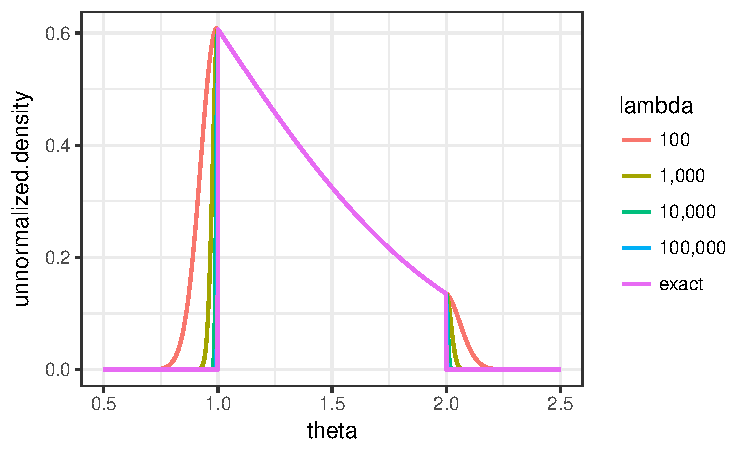
\includegraphics[width=0.5\textwidth]{density_truncated_normal}
\caption{Unnormalized densities for truncated normal $\No_{(-\infty,5)}(0,5^2)$ under exact intrinsic prior and approximating extrinsic prior. Inside $(-\infty,5)$, the priors are the same up to a constant difference. The intrinsic prior abruptly drops to $0$ on the boundary, while the approximating ones drop continuously. Intrinsic prior based on first-order $v(\theta)$ drops faster than the one based on second order when $v(\theta)\in (0,1)$.}
\label{truncated_normal}
\end{figure}


This smoothing function $\mc K(\theta;\mc D)$ in \eqref{smoothing} is applicable to more general and complicated scenarios. For example, $\theta$ can have some parameters constrained and some unconstrained; some parameters can be in multiple constraints simultaneously; constraints can be dependent. In all these cases, one can find proper $\mc D_k$'s and define $v_k(\theta)$'s accordingly.

\subsection{Property of Extrinsic Prior}

We now study the properties of the extrinsic prior. One important task is to quantify the difference between extrinsic and intrinsic priors. We first focus on the first case in \eqref{exact_prior1}, when $\int_{\mc D} \pi_{0,\mc R}(\theta)d\theta>0$.

%distance between extrinsic and intrinsic
\begin{remark}
Let $M_1= \int_{\mc D} \pi_{0,\mc R}(\theta)d\theta$ and $M_2 = \int_{\mc R} \pi_{0,\mc R}(\theta) \mc K(\theta;\mc D)d\theta$, when $M_1>0$, the total variation distance between the measures of extrinsic and intrinsic prior
$$||\pi_{0,\mc D}(\theta), \tilde{\pi}_{0,\mc D}(\theta) ||_{TV} = 1 - \frac{M_1}{M_2} \le \frac{\int_{\theta  \in \mc R \setminus \mc D} \pi_{0,\mc R}(\theta) \mc K(\theta;\mc D)d\theta}{M_1}$$.
\end{remark}
proof:
{via definition of total variation distance and $K(\theta;\mc D)=1$ when $\theta\in\mc D$, $0$ otherwise.}


In the case of exponential smoothing function \eqref{smoothing}, we have:
\begin{corollary}
Let $M_1= \int_{\mc D} \pi_{0,\mc R}(\theta)d\theta>0$ and $\mc K(\theta; D) = \prod_{k=1}^m \exp( -v_k(\theta)/\lambda_k)$, one sufficient condition to have
$$\lim_{\text{ all } \lambda_k\rightarrow 0}||\pi_{0,\mc D}(\theta), \tilde{\pi}_{0,\mc D}(\theta) ||_{TV} = 0$$
is that $\pi_{0,\mc R}(\theta)$ is proper, $\int_{\mc R} \pi_{0,\mc R}(\theta) d\theta<\infty$.
\end{corollary}
proof:
{via dominated convergence theorem}

Rewriting $\mc K(\theta; D) = \exp(-v(\theta)/\lambda)$ with $\lambda = \sup_k \lambda_k$, $v(\theta)=\lambda\sum_{k=1}^m\frac{ v_k(\theta)}{\lambda_k}$, we obtain the convergence rate:

\begin{remark}
Assuming $M_3= \int_{\mc R \setminus \mc D} \pi_{0,\mc R}(\theta) d\theta<\infty$, and $f(v)$ be the density of $v(\theta)$ as the transform of $\pi_{0,\mc R}(\theta)/M_3$. If there exists an $t<\infty$ such that $f(v) < \infty$ for $v<t$,
$$\int_0^\infty {\pi_{0,\mc R}(\theta)}exp(- \frac{v(\theta)}{\lambda}) d \theta \le 
2 {M_3} \exp(-\frac{t}{\lambda}) + {M_3} \sup_{t^*\in(0,t)} {f(t^*)}\lambda 
$$
\end{remark}
proof:

\begin{equation}
\begin{aligned}
\int_0^\infty {f(v)} \exp(- \frac{v}{\lambda}) d v
= & \int_0^t {f(v)} \exp(- \frac{v}{\lambda}) d v + \int_t^\infty {f(v)} \exp(- \frac{v}{\lambda}) d v \\
% \le &  t\frac{f(t^*)}{M_3} \exp(- \frac{t^*}{\lambda})+ \exp(- \frac{t}{\lambda})  \int_t^\infty \frac{f(v)}{M_3} d v \\
% \le &  t\frac{f(t^*)}{M_3} \exp(- \frac{t^*}{\lambda})+ \exp(- \frac{t}{\lambda})\\
\le & {F(t)} \exp(-\frac{t}{\lambda}) + 
\frac{1}{\lambda}\int_0^t {F(v)} \exp(-\frac{v}{\lambda})dv + \exp(-\frac{t}{\lambda}) \\
= & ({F(t)} +1) \exp(-\frac{t}{\lambda}) + 
\frac{1}{\lambda}\int_0^t {f(v^*)} v\exp(-\frac{v}{\lambda})dv \\
\le & ({F(t)} +1) \exp(-\frac{t}{\lambda}) + \sup_{t^*\in(0,t)} {f(t^*)}
\int_0^t  \frac{1}{\lambda}v\exp(-\frac{v}{\lambda})dv \\
\le & 2 \exp(-\frac{t}{\lambda}) + \sup_{t^*\in(0,t)} {f(t^*)}\lambda 
\end{aligned}
\end{equation}
where $F(t)=\int_0^t f(x)dx$ and the third step is based on mean value theorem with $v^*\in (0,v)$. Rearranging term yields the result.  $\blacksquare$

That is, for $\lambda$ small, the extrinsic prior approaches intrinsic prior in total varation distance in $O(\lambda)$. The rate is quantified under very general assumption. We expect it can be sharpened under special cases.

We now examine the second case in \eqref{exact_prior2} where ${ \int_{\mc D} \pi_{0,\mc R}(\theta)d\theta }=0$.


\leo{this needs some more work}
\begin{remark}
Let $M_1(\mc D^+)= \int_{\mc D^+} \pi_{0,\mc R}(\theta)d\theta$ and $M_2 = \int_{\mc R} \pi_{0,\mc R}(\theta) \mc K(\theta;\mc D)d\theta$, with $\mc D^+$ chosen such that $M_1(\mc D^+)>0$ and $M_1(\mc D^+)<M_2$, the total variation distance between the measures of extrinsic and intrinsic prior

$$||\pi_{0,\mc D}(\theta), \tilde{\pi}_{0,\mc D}      (\theta) ||_{TV} = 1 - \frac{\lim_{\mc D^+\supset \mc D}\int_{\theta  \in \mc D^+} \pi_{0,\mc R}(\theta) \mc K(\theta;\mc D)d\theta}{M_2} = \frac{\lim_{\mc D^+\supset \mc D}\int_{\theta  \in \mc R \setminus \mc D^+} \pi_{0,\mc R}(\theta) \mc K(\theta;\mc D)d\theta}{M_2}$$.
\end{remark}

\section{Posterior Computation}

Letting the likelihood function be $L(y;\theta)$, the posterior distribution of $\theta$ under a extrinsic prior is
\begin{equation}
\label{extrinsic_posterior}
	\tilde{\pi}_{\mc D}(\theta \mid y) = \frac{ L(y;\theta)\pi_{0,\mc R}(\theta) \mc{K}( \theta; \mc D) }{ \int_{\mc R} L(y;\theta)\pi_{0,\mc R}(\theta) \mc{K}(\theta; \mc D)d\theta },
\end{equation}
which we refer as extrinsic posterior from now on. As it is supported on a less restrictive space $\mc R$, one can exploit conventional sampling approach such as slice sampling, adaptive Metropolis-Hastings and Hamiltonian Monte Carlo (HMC) for posterior sampling. In this section, we focus on HMC for its easiness to use and good performance in sampling with high-dimensional parameter.

\subsection{Hamiltonian Monte Carlo for Extrinsic Posterior Sampling}

We first provide a short review of Hamiltonian Monte Carlo for continuous $\theta$, although discrete extension is possible \citep{zhang2012continuous,nishimura2017discontinuous}.

Assuming $\theta\in\mc R$, with $\mc R$ in a full or truncated Eucledean space $\mathbb R^d$. HMC augments a latent variable ``momentum'' $p\in \mathbb R^d$ (commonly generated from $\No(0, \Sigma)$ with $\Sigma$ pre-specified), ommiting constant, the negative log-posterior function based on \eqref{extrinsic_prior} is

% To be clear, this is different from Riemannian HMC that requires specific accommodation and heavy computation. The algorithm we use is simply conventional HMC in Euclidean space. In this section, we study the effects of choosing $\lambda$ on efficiency of Hamiltonian dynamics.

\begin{equation}
\begin{aligned}
H(\theta, p)& = U(\theta)+M(p),\\
\text{where } & U(\theta) = -\log\left\{ L(\theta;y)\pi_{0,\mc R}(\theta) \mc{K}(\theta;\mc D) \right\},\\
& M(p) = \frac{p'\Sigma^{-1} p}{2},\end{aligned}
\end{equation}
Denoting current state as $(\theta^{(0)},p^{(0)})$, HMC updates $\theta$ and $p$ via Hamiltonian dynamics, defined by two partial differential equations:

\begin{equation}
\begin{aligned}
\label{hamiltonian}
\frac{\partial \theta (t)}{\partial t} & =\frac{\partial H(\theta, p)}{\partial p} = \Sigma^{-1}p,\\
\frac{\partial p(t)}{\partial t}& =-\frac{\partial H(\theta, p)}{\partial \theta} = -\frac{\partial U(\theta)}{\partial \theta}.
\end{aligned}
\end{equation}

By evolving in $t>0$, this yields $(\theta^{(t)},p^{(t)})$. Since Hamiltonian system is symplectic, i.e. $H(\theta^{(t)},p^{(t)})=H(\theta^{(0)},p^{(0)})$, one can take $\theta^{(t)}$ as a new posterior sample. However, in most cases, \eqref{hamiltonian} lacks closed-form solution, one has to use an {\it integrator} that numerically approximates an evolution of the exact solution. With the integrator reversible and volume-preserving (see \citep{neal2011mcmc} for details), an Metropolis-Hastings (M-H) step is taken to correct the approximation error, by accepting $(\theta^{(t)},p^{(t)})$ with probability 
$$1\wedge \exp  \left( - H(\theta^{(t)},p^{(t)}) + H(\theta^{(0)},p^{(0)}))\right)$$

One common integrator is the leap-frog algorithm \citep{neal2011mcmc}that utilizes move $(\theta^{(T\epsilon)}, p^{(T\epsilon)}) \rightarrow (\theta^{((T+1)\epsilon)}, p^{((T+1)\epsilon)})$:

\begin{equation}
\begin{aligned}
\label{leap-frog}
p \leftarrow p - \frac{\epsilon}{2} \frac{\partial U}{\partial  \theta },\quad
 \theta \leftarrow  \theta  + \epsilon \Sigma^{-1}p,\quad
p \leftarrow p -  \frac{\epsilon}{2}  \frac{\partial U}{\partial  \theta } 
\end{aligned}
\end{equation}
for $T=0,\ldots,(L-1)$; where $L$ is the number of leap-frog steps within one iteration and $t=L\epsilon$.


\subsection{Optimizing Computing Efficiency}

As a Markov chain Monte Carlo, one would hope to use HMC to build a chain that rapidly converges. The convergence rate is associated with the maximal correlation  \citep{liu2008monte}, $\gamma (\theta,\theta^*) = \sup_{g \in L^2(\Pi)} \mbox{corr}(g(\theta), g(\theta^*))
$, where $L^2(\Pi)=\{g(\theta): \mbox{var}(g(\theta))<\infty\}$. Smaller $\gamma (\theta,\theta^*)$ corresponds to less correlation and faster convergence. At fixed $\epsilon$, one can adaptively choosing $L$ so that $\gamma (\theta,\theta^*)$ falls under certain desired rate \citep{hoffman2014no}.

We now further examine this via a view of computing efficiency. Since each iterator step is often the bottleneck, one would use as few steps as possible to reach below the desired convergence rate.  Given a desired convergence rate $\gamma^*$, an optimal $\epsilon$ would be:

$$\epsilon^* =  \underset{\epsilon: \epsilon \le \epsilon_{max}}{\arg\inf}\inf_{L}\{L: \gamma \left(\theta^{(0)}, \theta^{(\epsilon L)} \right) \le \gamma^*   \},$$
where $\epsilon_{max}$ is the stability bound for the integrator step size. Given fixed integrator time $\epsilon L$, to minimize $L$, often the optimality occurs when $\epsilon\approx \epsilon_{max}$.

The stability bound $\epsilon_{max}$ can be influenced by the specification in extrinsic prior. The stability bound is roughly determined by the width of distribution in the most constrained direction  \citep{neal2011mcmc}. To provide an intuition, we focus on one-step update $L=1$. Each update in leap-frog algorithm corresponds to $\theta^{(\epsilon)}=\theta^{(0)} + \epsilon  p^{(0)} - \epsilon^2/2  \frac{\partial U}{\partial  \theta } = \theta^{(0)} + \varepsilon  p^{(0)} + O(\epsilon^2)$. If the extrinsic posterior has support too narrow along certain direction, a random move in $\varepsilon  p(0)$ can end outside the support with $U(\theta^{(\epsilon)})=\infty$. This would violate the condition that discrete integrator approximately preserves $U(\theta^{(\varepsilon)})+M(p^{(\varepsilon)}) = U(\theta^{(0)})+M(p^{(0)})< \infty$.

Therefore to efficiently utilize HMC, if the constrained space $\mc D$ has narrow support via certain direction in its embedded space $\mc R$, one needs to create more relaxation in extrinsic prior. For example, one equality constraint $x+y+z=1$ in $\mathbb{R}^3$ creates a hyperplane. Extrinsic prior with $\exp(- \frac{|x+y+z-1|}{\lambda})$ relaxes the support along the normal vector of the plane, creating a slab with some thickness greater than $0$. To have decent $\epsilon_{max}$, one needs to avoid choosing $\lambda$ too small. Empirically, we found $\lambda= 10^{-3}$ is often a good value for such constraint.


\section{Examples and Application}

We now use examples to illustrate the properties of extrisinc priors and their utility in complex real data application.

We first illustrate the specification of tuning parameter and its effect in computational efficiency.  Consider data $y_i\in \mathbb{R}^2$ for $i=1,\ldots,n$  that are noisy realization from a unit circle:

$$y_i\sim \No(\theta_i, I_2\sigma^2),\text{ with } \theta_i'\theta_i=1,$$
where $\theta_i \in \mc V(2,1)$, in a $(2,1)$--Stiefel manifold, is assigned a von Mises--Fisher prior $\pi_{0,\mc D}(\theta) \propto \exp(F'\theta_i)$ with $\theta_i'\theta_i =1$. In generating data, we use $F=(1,1)$ to induce $\theta_i$ widely spreaded over the manifold and $\sigma^2=0.1^2$. For posterior sampling, we set $F$ to its oracle value and $\sigma^2$ unknown but associated with a inverse-Gamma prior $\text{IG}(2,1)$. To allow extrinsic posterior sampling, we use extrinsic prior $\tilde\pi_{0,\mc D}(\theta)= \exp(F'\theta_i) \exp(-\frac{|\theta'\theta -1|}{\lambda})$.

Geometrically, this prior expands the posterior support from a circle to a ring, with its width $|\theta'\theta -1|$ affected by $\lambda$.

\begin{figure}[H]
 \centering
    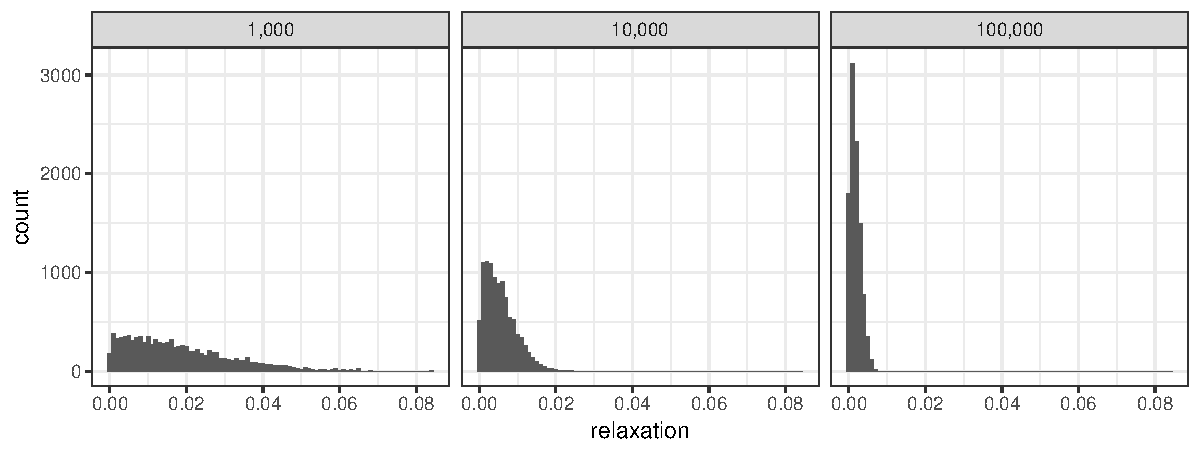
\includegraphics[width=0.8\textwidth]{unit_circle_violation}
  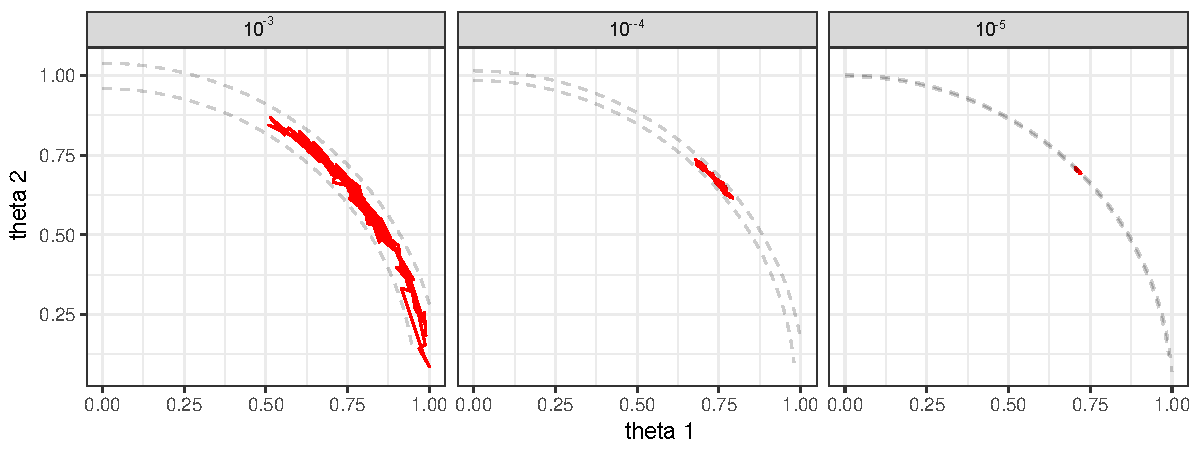
\includegraphics[width=0.8\textwidth]{unit_circle_100steps}
 % 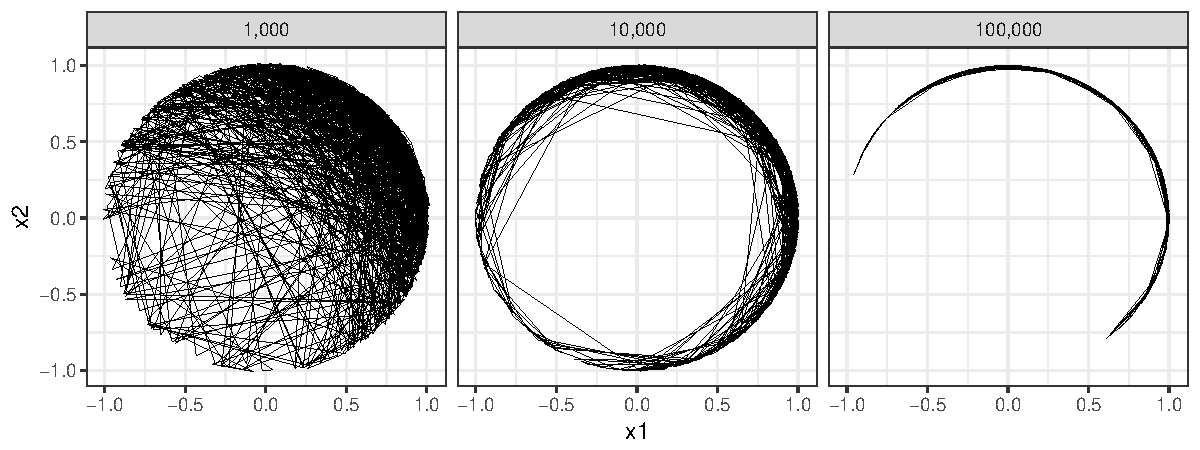
\includegraphics[width=0.8\textwidth]{unit_circle_path}
 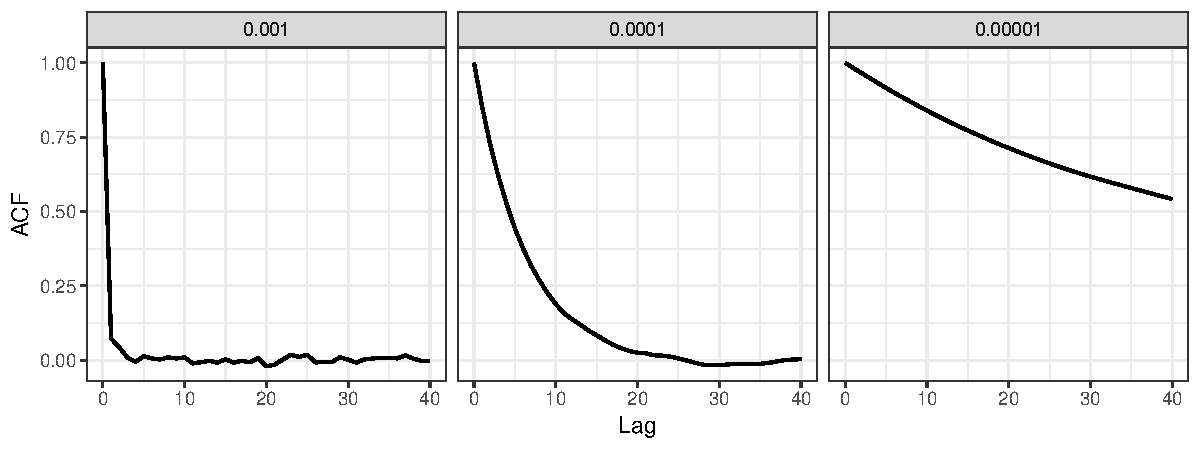
\includegraphics[width=0.8\textwidth]{unit_circle_acf}
\caption{Sampling posterior from a von Mises--Fisher distribution on a unit circle, using HMC with extrinc prior under $\lambda=10^3,10^4,10^5$. Row $1$ shows the posterior distribution of the constraint relaxation $|\theta'\theta -1|$; Row $2$ shows the path of $100$ leap-frog steps; Row $3$ shows the autocorrelation plot (ACF). Large $\lambda$ gives very small constraint relaxation, but suffers from slow mixing due to inefficient local update; smaller $\lambda$ increases the relaxation but results in excellent mixing.}
\label{unit_circle}
\end{figure}


We tested three different values of $\lambda = 10^3,10^4,10^5$. For each $\lambda$, we ran HMC for $10,000$ iterations, with $L=100$ leap-frog steps in each iteration. 
We set $\Sigma= \diag(1,1)$ in generating velocity $p$. During the initial $2,000$ iterations, the leap-frog step size $\varepsilon$ is tuned for an acceptance rate close to $0.8$, then it is fixed during the remaining part of Markov chain. The last $5,000$ iterations are used as posterior samples. Figure~\ref{unit_circle} plots the posterior distribution of constraint relaxation $|\theta'\theta -1|$, the sampling path and the autocorrelation function (ACF) for each Markov chain. Very large $\lambda=10^5$ has much less constraint relaxation; however, due to the small ring width, the Hamiltonian dynamics has to use small $\varepsilon$ and can only explore local space for each $100$ time steps. This results in a very slow mixing (large autocorrelation even at 40 lags). On the other hand, smaller $\lambda=10^3$ has slightly larger constraint relaxation, but allows much more efficient exploration of the space and excellent mixing performance. In general, we find that $\lambda=10^3$ is a good empirical value for all the equality constraints used in this paper.


In this section, we demonstrate the utility of extrinsic prior via three examples. %Through the simple implementation of equality and inequality in the prior, our approach not only works well with conventional constrained model such as probability simplex, but also allows low-cost inclusion of additional constraints, which are useful to improve computational efficiency.

{\bf Example 1: Ordered Dirichlet Prior in Mixture Model}

We first consider a simplex modeling problem, where a $(J-1)$--simplex $w=\{w_1,\ldots w_J\}$ has all $w_j\in (0,1)$ and $\sum_{j=1}^J w_j=1$. We illustrate its use via a normal mixture model with mixture means and common variance, for data $y_i\in \bb R^d$ indexed by $i=1,\ldots,n$:

\begin{equation*}
\begin{aligned}
y_i &\stackrel{indep}{\sim} \No(\mu_i,\Sigma),\\
\mu_i &\stackrel{iid}{\sim} G,\\
G(.) & = \sum_{j=1}^{J} w_j \delta_{\mu_j}(.),
\end{aligned}
\end{equation*}
which is associated with likelihood
\begin{equation*}
\begin{aligned}
L(y) = |\Sigma|^{-n/2}\prod_{i=1}^n \sum_{j=1}^{J} w_j \exp\left(-\frac{1}{2}{ (y_i-\mu_j)'\Sigma^{-1}(y_i-\mu_j)}\right).
\end{aligned}
\end{equation*}

Standard practice assigns Dirichlet distribution on the simplex in finite mixture $Dir(\alpha)$ and Dirichlet process $DP(\alpha)$ for infinite mixture when $J$ is unknown. For simplicity, we focus on finite mixture case with $J$ finite and known. The prior $Dir(\alpha)$ can be viewed as a prior $\pi_{0, \mc R}(w) = \prod_{j=1}^J w_j^{\alpha-1}$ with $\mc R = (0,1)^J$, under additional hard constrained of $1-$norm equality:

\begin{equation}
\begin{aligned}
\label{canonical_dp_prior}
\pi_{0, \mc D}(w) \propto \prod_{j=1}^J w_j^{\alpha-1} \1_{\sum_{j=1}^J w_j=1}
\end{aligned}
\end{equation}

This can be easily approximated with extrinsic prior. However, one known issue for mixture modeling under canonical Dirichlet prior is the label-switching problem. With parameter $\{\mu_j,w_j\}$ indexed by $j=1,\ldots,J$, due to exchangability, one can switch any two $j$ and $j'$ without changing likelihood. It is a controversial topic whether the occurrence of label-switching or the lack thereof is more ideal (see review in \cite{jasra2005markov}) in general; but in the case that posterior distribution is symmetric about any permutation in $j$'s, as our normal mixture example, sampling over all permutations of $j$ is redundant. Therefore, it is rather useful to avoid label-switching and have convergence in such cases. Unfortunately, sometimes the switching issue can be impossible to avoid, even with very local update in Gibbs sampling. This is because when sample size $n$ is small, posterior variances of $\mu_j$'s can be quite large, with significant overlap among their high posterior regions. In early work, \cite{diebolt1994estimation} suggested ordering in $\mu_j$'s, but it is not clear how it would work with multi-dimensional $\mu_j\in \bb R^d$ with $d\ge 2$.

Observing that each $w_j$ is one-dimensional, we apply order constraint on $w_1 \ge w_2 \ge \ldots \ge w_J$, yielding an ordered Dirichlet prior:

 \begin{equation}
\begin{aligned}
\label{ordered_dp_prior}
\pi_{0, \mc D}(w_1,\ldots w_J) \propto \prod_{j=1}^J w_j^{\alpha-1} \cdot \1_{\sum_{j=1}^J w_j=1} \cdot  \prod_{j=1}^{J-1}\1_{w_j \ge w_{j+1}}.
\end{aligned}
\end{equation}
where $w_j\in (0,1)$. Unlike early post-hoc relabeling algorithm \citep{stephens2000dealing}, we remove exchangability directly to reduce label-switching. Strictly speaking, label-switching could still happen when any two $w_j$'s are very close; nevertheless, this help prevent label-switching between large and small components.

The ordered Dirichlet no longer has closed-form posterior, however it is easy to approximately estimate with the help of extrinsic prior:

 \begin{equation*}
\begin{aligned}
\pi_{0,\mc R}(w)\cdot \mc K(w) \propto \prod_{j=1}^J w_j^{\alpha-1} \cdot \prod_{j=1}^{J-1} K_{1}{\left(( w_{j+1} - w_j )_+\right)} \cdot K_2 ( |{\sum_{j=1}^J w_j - 1}|)
\end{aligned}
\end{equation*}
where $K_{k}(x)=\exp(- \lambda_k x^2) \1_{x<4/\sqrt{2\lambda_k}}$ for  $k=1,2$. We use $\lambda_1 = 10^6$ to induce almost no relaxation on the ordering and $\lambda_2 = 10^3$ to allow efficient mixing in embedding a simplex in $\mathbb{R}^J$. For comparison, we also test with $\lambda_1=0$ to remove the order constraint and allow HMC to run on a canonical Dirichlet prior in \eqref{canonical_dp_prior}.

We generate $n=100$ samples from $3$ components with true $\{w_1,w_2,w_3\}=\{0.6,0.3,0.1\}$, with corresponding two-dimensional means $\{\mu_1,\mu_2,\mu_3\} = \{[1,5], [3,3], [3,5]\}$ and identity covariance $\Sigma = I_2$. We assign informative priors $\No(0,10 I_2)$ for each $\mu_j$ and inverse Gamma prior for the digonal element in $\Sigma=\diag(\sigma_1^2,\sigma_2^2)$ with $\sigma^2_1, \sigma^2_2\sim IG(2,1)$.  

Figure~\ref{dirichlet} shows the contour of true posterior density of $\mu_j$'s and the traceplot of $w_j$'s in three approaches: standard Gibbs sampling with augmented component assignment \citep{diebolt1994estimation} under canonical prior \eqref{canonical_dp_prior}, HMC using extrinsic prior associated under canonical  prior \eqref{canonical_dp_prior} and and HMC using extrinsic prior under ordered prior \eqref{ordered_dp_prior}. Each approach runs $10,000$ iterations with first $5,000$ discarded as burn-in. For the posterior extrinsic collected under extrinsic prior, a simple projection $P(w^*)=w^*/||w^*||_1$ is used as proposal in M-H correction, yielding acceptance rate of $0.95$. Due to small sample size and relatively overlap of means, significant label-switching is shown in both Gibbs and HMC under canonical Dirichlet prior; while HMC with ordered Dirichlet prior does not suffer this issue.



\begin{figure}[H]
\begin{center}
   \begin{subfigure}[b]{0.3\textwidth}
    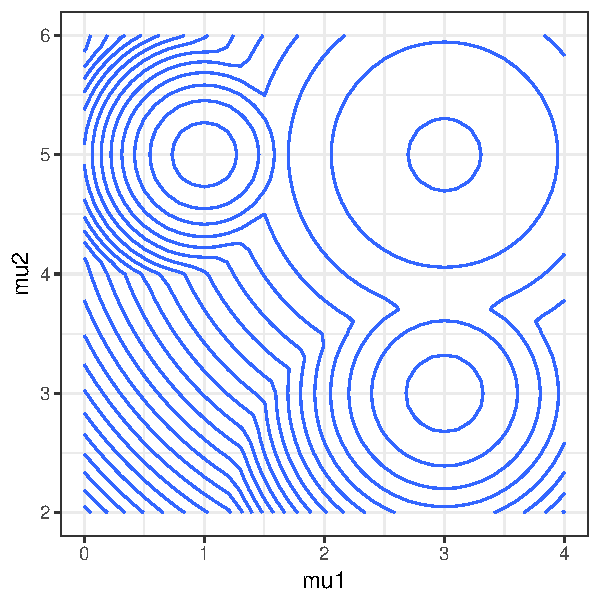
\includegraphics[width=1\textwidth]{fmm_mu_contour.pdf}
    \caption{Posterior density of the component means.}
    \end{subfigure}
    \end{center}
    \centering
   \begin{subfigure}[b]{0.32\textwidth}
    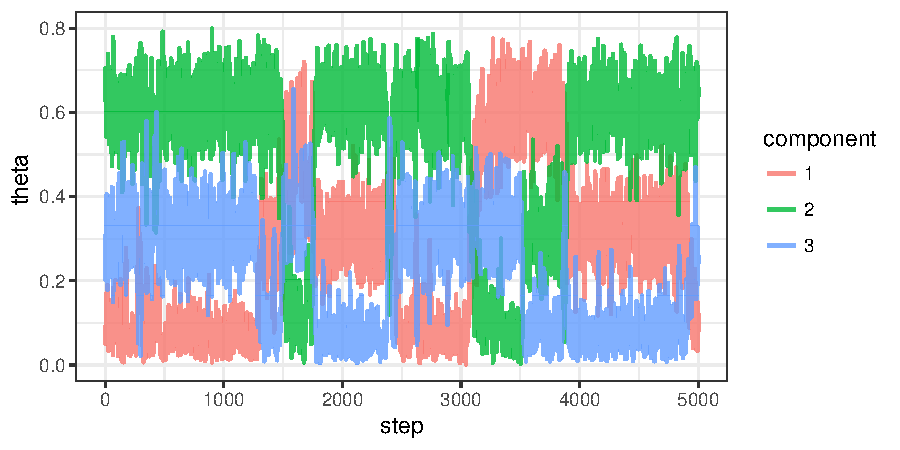
\includegraphics[width=1\textwidth]{fmm_w_gibbs.pdf}
    \caption{Gibbs sampling under canonical Dirichlet}
    \end{subfigure}
       \begin{subfigure}[b]{0.32\textwidth}
  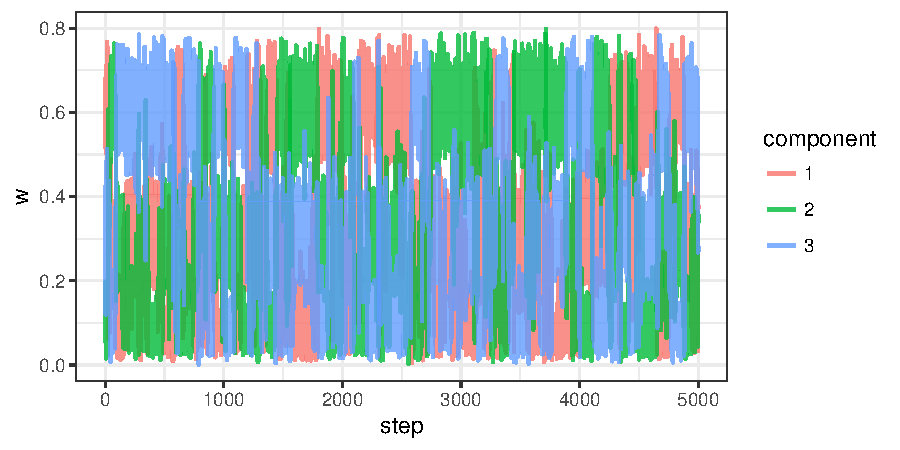
\includegraphics[width=1\textwidth]{fmm_w_hmc_unordered.pdf}
    \caption{HMC sampling under canonical Dirichlet, using extrinsic prior}
      \end{subfigure}
       \begin{subfigure}[b]{0.32\textwidth}
 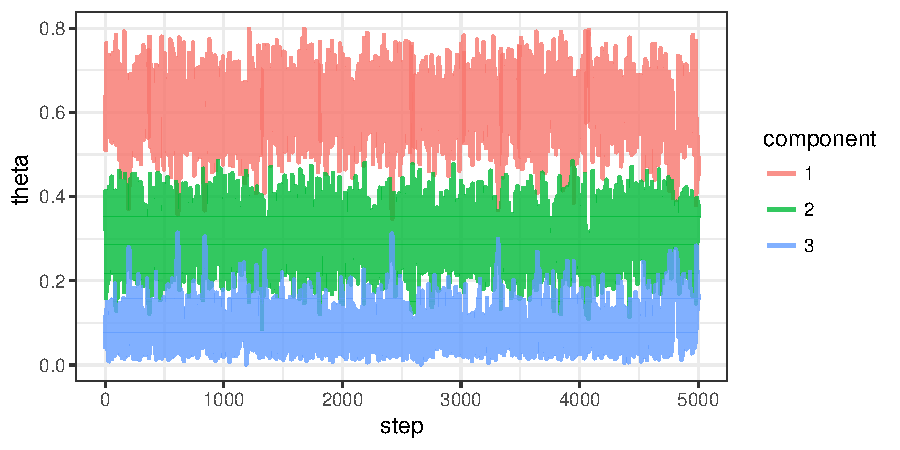
\includegraphics[width=1\textwidth]{fmm_w_hmc.pdf}
     \caption{HMC sampling under ordered Dirichlet, using extrinsic prior}
     \end{subfigure}
\caption{Contour of the posterior density of component means and traceplot of the posterior sample for the component weights, in a 3-component normal mixture model. Panel (a) shows that there is significant overlap among component means, creating label-switching issues in both Gibbs sampling (b) and HMC sampling using canonical prior (c). The ordered Dirichlet prior, estimated under extrinsic prior and correcting projection, significantly reducing label-switching (d).}
\label{dirichlet}
\end{figure}


%{\bf Example 2: Orthonormal Gaussian Processes in Functional Principle Component Analysis}
%
%\leo{There are some issues with this model. Skip it for now.}
%
%We now consider functional principle component analysis. Letting $x_i$ be the input for $i=1,\ldots,n$ in functions $f_j(x_i)$ for $j=1,\ldots,p$. We observe functional data $y_{i,j}$ as noisy realizations of $f_j(x_i)$. Commonly, $p$ is very large and it is useful to view the functions as linear combination of $d$ functional factors $g_k$.
%
%\begin{equation*}
%\begin{aligned}
%y_{ij} & = f_j(x_i) + \epsilon_{ij},\\
% f_j(x_i) & = \sum_{k=1}^{d} \eta_{jk} g_k(x_i),\\
% \left [ g_k(x_1) , \ldots , g_k(x_n) \right] &\sim \No (0, \Sigma_k)\\
%\Sigma_{k,(i,i')} &= \phi_k\exp( - \frac{||x_i-x_{i'}||^2}{2\rho_k^2})
%\end{aligned}
%\end{equation*}
%for $k=1,\ldots d$ with $d<p$, and $\epsilon_{ij}\sim \No(0,\sigma^2)$ is the random measurement error; $\Sigma_{k,(i,i')}$ is the $(i,i')$th element in matrix $\Sigma_k$. Using matrix notation $G=[g_1, \ldots, g_d]$ and $\eta= [\eta_{.1},\ldots,\eta_{.d}]$, the $n\times p$ function matrix $[f_j(x_i)]_{ij}$ can be written as $G \eta'$. We utilize a squared exponential Gaussian process to model each latent factor $g_k$.
%
%We first assign a shrinkage prior on loadings $\eta_{jk}\sim \No(0,\tau_k)$, $\tau_k \sim IG(aq^{3(k-1)},q^{2(k-1)})$  with $q>1$. This prior ensures the shrinkage grows stronger as $k$ increases \citep{bhattacharya2011sparse}, avoiding arbitrary specification of $d$ and exchangability in permuting $k$. However, $G$ and $\eta$ are still not identifiable. Any orthonormal matrix $P$ that $P'P = I_d$ can produce another set of factors $G^*= GP'$ and loadings $\eta^* = P\eta$. Since this projection $P$ is associated with rotation, scaling or column-wise sign change, we apply the following constraint on $G$:
%
%\begin{equation*}
%\begin{aligned}
% \sum_{i=1}^n g_k(x_i) g_{k'}(x_i) &= \left\{ \begin{array}{cc}1 \text{ if } k=k' \\ 0 \text{ if } k \neq k'\end{array}\right. \\
% g_k(x_1) \ge 0
%<<<<<<< HEAD
%\end{aligned}
%\end{equation*}
%for $k=1,\ldots d$. The orthonormailty restricts rotation and scaling and $g_k(x_1)\ge 0$ restricts column-wise sign change. 
%
%As the result, these constraints create a Gaussian process prior on a Stiefel manifold $\mc V(N,d)$. To our best knowledge, this is the first application of Gaussian process in this manifold. We approximate these constraints with extrinsic prior:
%
% \begin{equation*}
%\begin{aligned}
%\pi_{\mc K}(G) \propto   \prod_{k=1}^{d} K_{1}{\left((-g_k(x_1) )_+\right)} \cdot \prod_{k'=1}^{d}\prod_{k=1}^{k'} K_2 ( |\sum_{i=1}^n g_k(x_i) g_{k'}(x_i) - \delta_{k,k'}|)
%\end{aligned}
%\end{equation*}
%where $K_{k}(x)=\exp(- \lambda_k x^2) \1_{x<4/\sqrt{2\lambda_k}}$ for  $k=1,2$. We use $\lambda_1 = 10^6$ to strongly enforce the sign of $g_k(x_1)$ to be positive, while $\lambda_2 = 10^3$ to allow efficient mixing in embedding Stiefel manifold in $\mathbb{R}^{N\times d}$. To compare with unconstrained Gaussian processes for $g_k$'s, we also test with $\lambda_1=0$ and $\lambda_2=0$.
%
%We generate $n=50$ inputs $x_i\sim \text{U}(0,1)$ from uniform $(0,1)$ and three smooth functions $g^*_1(x)= \sin(16 x)/x$, $g^*_2(x)= \sin(25 x)\cdot x$ and $g^*_3(x)= \cos(20 x)/x$. The functions are combined via $f_j(x_i)=\sum_{i=1}^3 \eta^*_{jk} g^*_k(x_i)$ with $\eta^*_{jk}\stackrel{iid}{\sim} \No(0,1)$ for $j=1,\ldots,20$ and $i=1,\ldots,n$. We add random noise to create a $50\times 20$ data points $y_{ij} \sim \No(f_j(x_i),0.1^2)$, and randomly remove $20\%$ of data to mimic the unbalanced data in real world. We set $a=q=2$ in the shrinkage prior for all $\eta_{jk}$'s, uniform prior $\text{U}(0,20)$ for all $\rho_k$'s, $\phi_k$'s and $\sigma^2$.

{\bf Example 2: Orthonormal Tucker Factorization in Multiple Network Analysis}

We now consider another application of constrained model in network analysis. What a a


 \begin{equation*}
\begin{aligned}
& A_i \sim \text{Bern}( \frac{1}{1+ \exp(- \psi_i)})\\
& \psi_i = UD_iU \\
& D_i = \diag(d_{i1},d_{i2},d_{i3}) \\
& vec(U) \sim N (vec (X), \sigma^2)\\
\end{aligned}
\end{equation*}
for $k=1,\ldots d$. The orthonormailty restricts rotation and scaling and $g_k(x_1)\ge 0$ restricts column-wise sign change. 



\section{Discussion}



\bibliography{reference}
\bibliographystyle{chicago}

\end{document}



We now illustrate a curve fitting problem where the shape of curve is convex. Convexity is common in real life such as a trajectory of projectile or accelerated decreasing of organ functions in disase monitinoring. Consider a cubic spline function $f(t)$ for data $y_t$ with $t\in [0,1]$


\begin{equation*}
\begin{aligned}
y_t & = f(t) + \epsilon_t,\\
f(t) & = \beta_0 + \beta_1 t + \beta_2 t^2+ \beta_3 t^3+ \sum_{j=1}^J b_j (t- \tau_j)^3_+,\\
\end{aligned}
\end{equation*}
where $\epsilon_t \sim \No(0, \sigma^2)$ and $\tau_j$'s are pre-specified knots in $(0,1)$. To induce the convexity, it suffices to have the second derivative:

\begin{equation*}
\begin{aligned}
f''(t) & =  2\beta_2 + 6\beta_3 t+ \sum_{j=1}^J 6b_j (t- \tau_j)_+ \ge 0.\\
\end{aligned}
\end{equation*}

Given data $y_t$ at observed time $t=t_1,\ldots, t_n$, the posterior estimation of $\beta_.$ and $b_.$ is estimated under $n$ linear inequality constraints.

